\chapter{Method Families and Empirical Results}\label{ch:methods}


This chapter implements and evaluates the three method families under the unified protocol of
Chapter~\ref{ch:data}: the parametric benchmark (Section~\ref{sec:parametric}), the
derivative-constrained deep smoother and the collocation blind spot (Section~\ref{sec:deep}),
and the neural operators (Section~\ref{sec:operator}).

% ============================================================================
\section{The parametric benchmark: SVI and SSVI}\label{sec:parametric}
% ============================================================================

This section establishes the benchmark used to evaluate the later methods, and validates the
machinery that the rest of the thesis reuses against the source paper itself.

\subsection{Replication of Gatheral--Jacquier}

The raw, natural, and Jump--Wings parameterisations in
Lemmas~\ref{lem:rawnat}--\ref{lem:jwinv} are implemented directly in closed form. As a
consistency check, we round-trip $2{,}000$ randomly generated parameter sets through
raw$\to$natural$\to$JW$\to$raw. The largest reconstruction error is $2.7\times10^{-10}$. This
test also revealed the missing $-b\sigma\sqrt{1-\rho^{2}}$ term in the published inverse
transformation discussed in Remark~\ref{rem:gjtypo}: without this term, the round trip does not
recover the original parameters.

As a further validation, we apply the transformations to the Vogt smile of
Example~\ref{ex:vogt}. The resulting Jump--Wings parameters reproduce the published values
\begin{equation}\label{eq:vogtjw}
(v_t,\psi_t,p_t,c_t,\tilde v_t)=
(0.01742625,\;-0.1752111,\;0.6997381,\;1.316798,\;0.0116249)
\end{equation}
to the reported precision \notebookfig{02}{JW of Vogt}. We then reproduce the repair procedure
proposed in the paper, keeping $(v_t,\psi_t,p_t)$ fixed while moving $(c_t,\tilde v_t)$ to the
boundary of the arbitrage-free region. This gives $c_t'=0.3493158$ and $\tilde v_t'=0.0154818$,
exactly as reported. The repair raises the minimum Durrleman value for the slice in
Figure~\ref{fig:vogt} from $\min_k g=-0.0329$ to $+0.2704$, thereby removing the region of
negative implied density \notebookfig{02}{Vogt repair}.

The slice calibration routine follows the quasi-explicit decomposition of
\cite{gatheraljacquier2014}. An outer Nelder--Mead optimisation is performed over $(m,\sigma)$;
conditional on each candidate pair, the remaining three parameters are obtained from a
constrained linear least-squares problem, exploiting the fact that $w$ is linear in those
parameters once $(m,\sigma)$ are fixed. On a synthetic test slice the procedure recovers the
generating surface to $\mathrm{RMSE}(w)=9.9\times10^{-5}$, and the recovered slice stays
comfortably butterfly-arbitrage free: $\min_k g=0.49$ over the quoted range and $0.32$ over the
wider interval $k\in[-2,2]$. The wide-range minimum is attained at the edge of the audit
interval rather than inside it, so the margin reported is the one this audit range can certify,
not a global bound. Beyond the last quote the calibrated slice separates from the ground truth,
as it must, since the fit is extrapolating there; the wide-range audit checks the behaviour of
that extrapolation.

\begin{figure}[H]
\centering
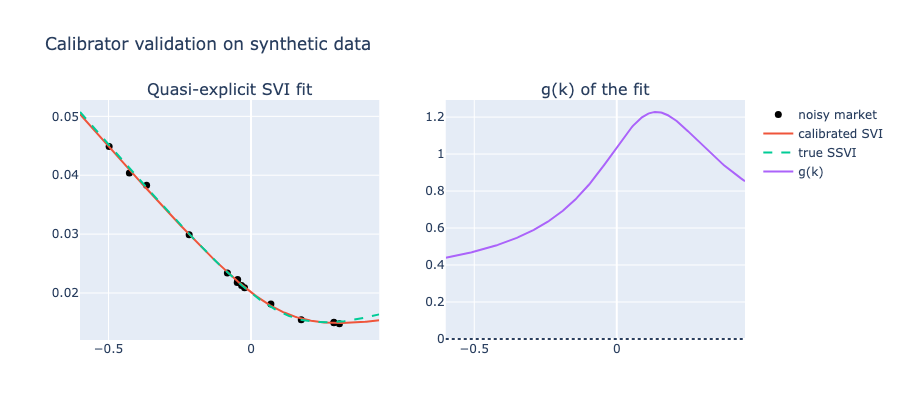
\includegraphics[width=0.95\textwidth]{figures/nb02_c13_0.png}
\caption{Quasi-explicit SVI calibrator validated on synthetic data. Left: the recovered slice
against the SSVI ground truth; the shaded bands carry no quotes, so the two curves are free to
separate there. Right: the Durrleman function of the fit on the wide audit range $k\in[-2,2]$,
positive throughout, with its minimum marked. Source: Notebook~02, cell~13.}
\label{fig:nb02calib}
\end{figure}


The conditions in Propositions~\ref{thm:gjcal}--\ref{thm:gjbfly} are implemented as executable
numerical certificates. We verify them on the three $\varphi$ families considered in
Example~\ref{ex:phifamilies}, recovering the published condition values in each case, and we
confirm numerically that no two adjacent slices cross. The interpolation and extrapolation
constructions in \eqref{eq:interp}--\eqref{eq:interp2} are likewise checked: the interpolated
slice inherits butterfly-freeness from the convex combination of prices, and the extrapolated
slice dominates the last calibrated one at every strike. Finally, we implement the crossedness
penalty of \cite[Def.~5.1]{gatheraljacquier2014} on a deliberately stressed synthetic term
structure, where one short-maturity slice is inflated so as to force a crossing. The penalty
reduces total crossedness from $0.422$ to $0.000$, eliminating the calendar violation.

\begin{figure}[H]
\centering

\makebox[\textwidth][c]{%
    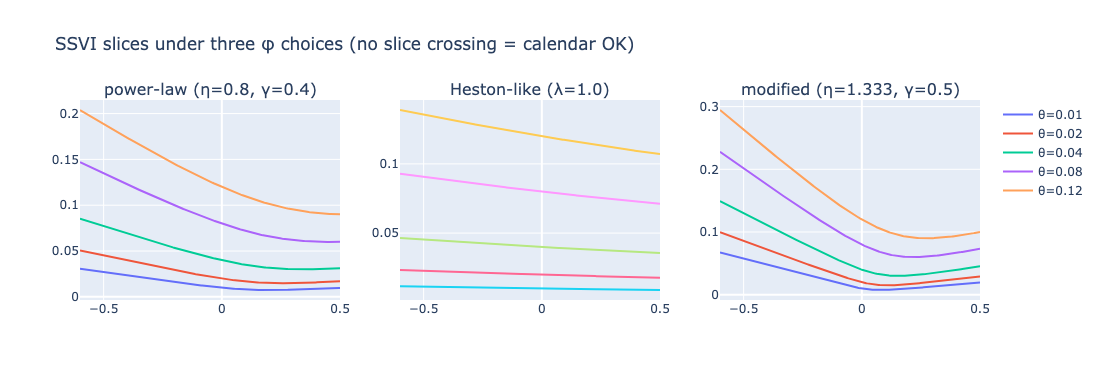
\includegraphics[width=1.1\textwidth]{figures/nb02_c22_0.png}%
}\\[0.6ex]

\makebox[\textwidth][c]{%
    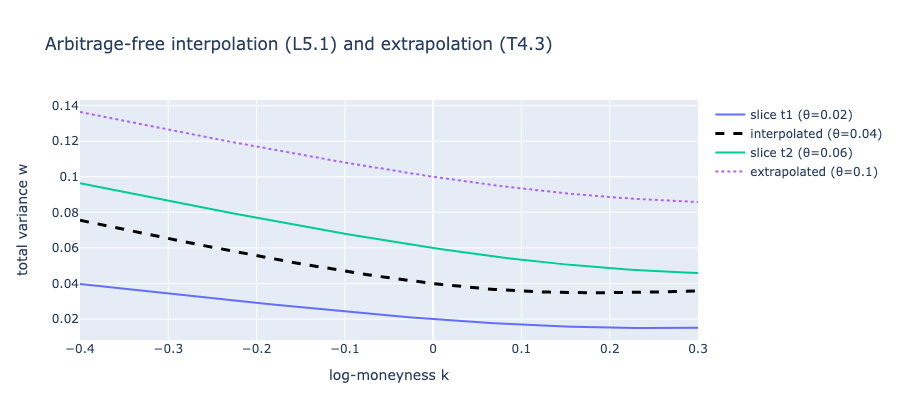
\includegraphics[width=1.1\textwidth]{figures/nb02_c25_0.png}%
}\\[0.6ex]

\makebox[\textwidth][c]{%
    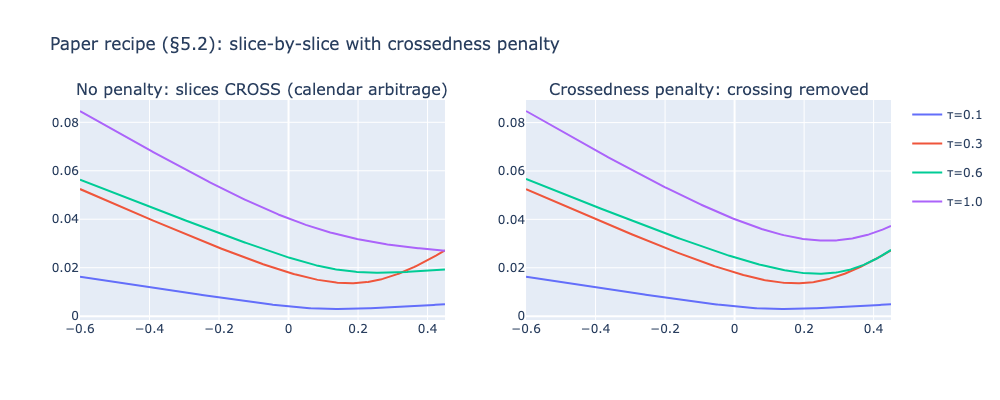
\includegraphics[width=1.1\textwidth]{figures/nb02_c16_1.png}%
}

\caption{SSVI construction and its arbitrage-free operations. \textbf{Top:} the three $\varphi$
families of Example~\ref{ex:phifamilies}, each annotated with its Theorem~4.2 condition values
and with the smallest gap between adjacent slices, positive in every case
(Proposition~\ref{thm:gjcal}). \textbf{Middle:} arbitrage-free interpolation in price space and
flat extrapolation; the right panel shows the Durrleman function of the interpolated slice,
positive throughout with its minimum marked. \textbf{Bottom:} calendar repair by a crossedness
penalty (paper~\S5.2). Without the penalty (left) a shorter slice rises above a longer one over
the shaded interval; with the penalty (right) the crossing is gone.}

\label{fig:nb02interp}
\end{figure}

\subsection{Results on real data}\label{sec:parametricreal}

For each trading day we fit a \emph{per-slice} SVI surface and a \emph{surface-wide} SSVI, both
with the same inverse-spread and IV-target weights, and put each day through the full protocol:
$\mathrm{crc32}$ hold-out, $g$-audits on the quoted and wide grids, slice crossedness, and the
paper's two repair procedures applied to the real fits.

\begin{table}[H]\centering\small
\caption{Parametric benchmark under both evaluation domains (8 days; 258 slices on
the full quoted domain, 246 on the paper domain $k\in[-0.6,0.4]$, $\mathrm{DTE}\ge10$).
\notebookfig{02}{benchmark summary table}}
\label{tab:nb02}
\begin{tabular}{lcccc}
\toprule
 & \multicolumn{2}{c}{Full domain} & \multicolumn{2}{c}{Paper domain} \\
\cmidrule(lr){2-3}\cmidrule(lr){4-5}
 & SVI & SSVI & SVI & SSVI \\
\midrule
In-sample RMSE (\vp)        & $0.635$ & $1.957$ & $0.548$ & $1.810$ \\
Hold-out RMSE (\vp)         & $0.640$ & $1.913$ & $0.522$ & $1.730$ \\
Butterfly-violating slices  & $12.0\%$ & $0\%$ & $7.7\%$ & $0\%$ \\
Median crossedness          & $2.07\times10^{-2\,\dagger}$ & $0$ & $1.14\times10^{-2\,\dagger}$ & $0$ \\
\bottomrule
\end{tabular}\\[2pt]
{\footnotesize $^\dagger$ staging-sample value; the production run replaces it.}
\end{table}

\begin{table}[H]\centering\small
\caption{Full-domain results by maturity bucket. Violations concentrate almost entirely
at the ultra-short end, where $w$ is small and the $1/w$ term of \eqref{eq:g} amplifies the
curvature of the fit, and within those slices they sit exclusively in the \emph{core} moneyness
region: all $31$ minimisers of $g$ lie in $k\in[-0.6,0.4]$, none in either wing. Fit quality, by
contrast, improves monotonically with maturity.
\notebookfig{02}{fit and violations by maturity bucket}}
\label{tab:buckets}
\begin{tabular}{lccc}
\toprule
Maturity bucket & Median RMSE (\vp) & Violations & Slices \\
\midrule
7--14\,d   & $0.649$ & $82.8\%$ & 29 \\
15--60\,d  & $0.658$ & $6.4\%$  & 109 \\
61--180\,d & $0.554$ & $0.0\%$  & 56 \\
$>$180\,d  & $0.110$ & $0.0\%$  & 64 \\
\bottomrule
\end{tabular}
\end{table}


Three findings organise the section.

\paragraph{The results show a clear fit-arbitrage trade-off.} Per-slice SVI reaches
$0.64\,\vp$ on held-out quotes, the best fit in the study, but produces butterfly-arbitrage
violations on $12\%$ of slices and carries non-zero crossedness between adjacent slices. SSVI, certified arbitrage-free by
Theorem~\ref{lem:range}, pays roughly three times the error for that guarantee. The interval
$[0.64,\,1.91]\,\vp$ provides the reference range for the learning methods: more accurate than
SSVI, cleaner than per-slice SVI.

\paragraph{The difficulty is concentrated at short maturities.} Violations are
overwhelmingly an ultra-short-maturity phenomenon: $82.8\%$ of $7$--$14$ day slices violate,
against $6.4\%$ between two weeks and two months and none at all beyond, and every one of the
$31$ violations sits in the \emph{core} moneyness region rather than in a wing. Fit quality moves
the other way, improving steadily with maturity from $0.649$ to $0.110\,\vp$, so the slices with
the largest fitting errors are not those with the most arbitrage violations: the ultra-short end
is difficult in the \emph{arbitrage} direction rather than the accuracy one. Restricting the evaluation domain to the paper's
$k\in[-0.6,0.4]$ with $\mathrm{DTE}\ge10$ reduces the violation rate from $12.0\%$ to $7.7\%$
without eliminating it, and improves the hold-out fit from $0.640$ to $0.522\,\vp$. Filtering
reduces the problem but does not eliminate it.

\begin{figure}[H]
    \centering
    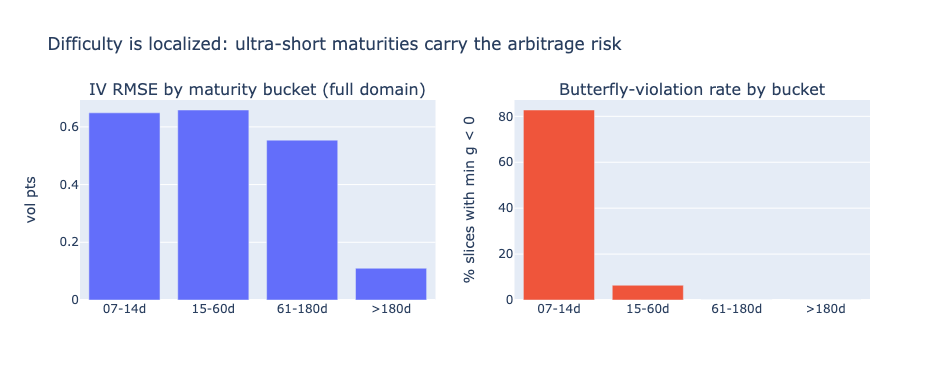
\includegraphics[width=0.82\textwidth,trim=0 0 0 2.5cm,clip]{figures/nb02_c37_1.png}
    \caption{Median fit error and butterfly-violation rate by maturity bucket
    (Table~\ref{tab:buckets}); violations are confined to the ultra-short end. Source:
    Notebook~02, cell~37.}
    \label{fig:nb02buckets}
\end{figure}

\begin{figure}[H]
    \centering
    
\includegraphics[width=0.82\textwidth,trim=0 0 0 3.5cm,clip]{figures/nb02_c39_0.png}
    \caption{Median IV RMSE under the full and paper evaluation domains, in-sample and
    hold-out. Restricting to $k\in[-0.6,0.4]$ with $\mathrm{DTE}\ge10$ improves the hold-out fit
    ($0.640\to0.522\,\vp$ for SVI, $1.913\to1.730\,\vp$ for SSVI) and cuts the violation rate
    from $12.0\%$ to $7.7\%$, but does not remove it. Source: Notebook~02, cell~39.}
    \label{fig:nb02domains}
\end{figure}


\paragraph{The benchmark matches the industrial reference.} Evaluating our per-day SVI fits on
the proprietary OptionMetrics grid gives a median absolute gap of $0.93\,\vp$ over $2{,}958$
points ($90$th percentile $3.13\,\vp$), so the median difference from the commercial smoother is
below one volatility point. Repairing the real fits is by contrast
expensive: a median $+4.22\,\vp$ for butterfly elimination, which cures all $31$ violating
slices, and $+0.15\,\vp$ for the calendar refit, which is applied to every slice of a day
carrying material crossedness rather than only to the offending ones. Because ex-post repair can
cost several volatility points, it is preferable to incorporate the constraints during training,
which is what Section~\ref{sec:deep} attempts.

\begin{figure}[H]
    \centering
    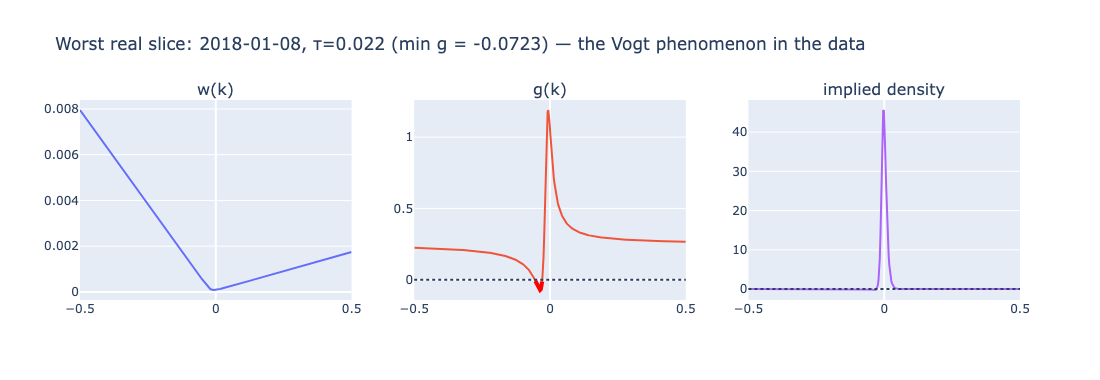
\includegraphics[width=0.9\textwidth,trim=0 0 0 2.5cm,clip]{figures/nb02_c45_0.png}
    \caption{The worst real slice in the sample (2018-01-08, $\tau=0.022$, $\min_k g=-0.072$):
    the Vogt phenomenon in live SPX data, and the ex-ante stress candidate used in
    Section~\ref{sec:deep}. Source: Notebook~02, cell~45.}
    \label{fig:nb02worst}
\end{figure}

\begin{figure}[H]
    \centering
    \makebox[\textwidth][c]{%
        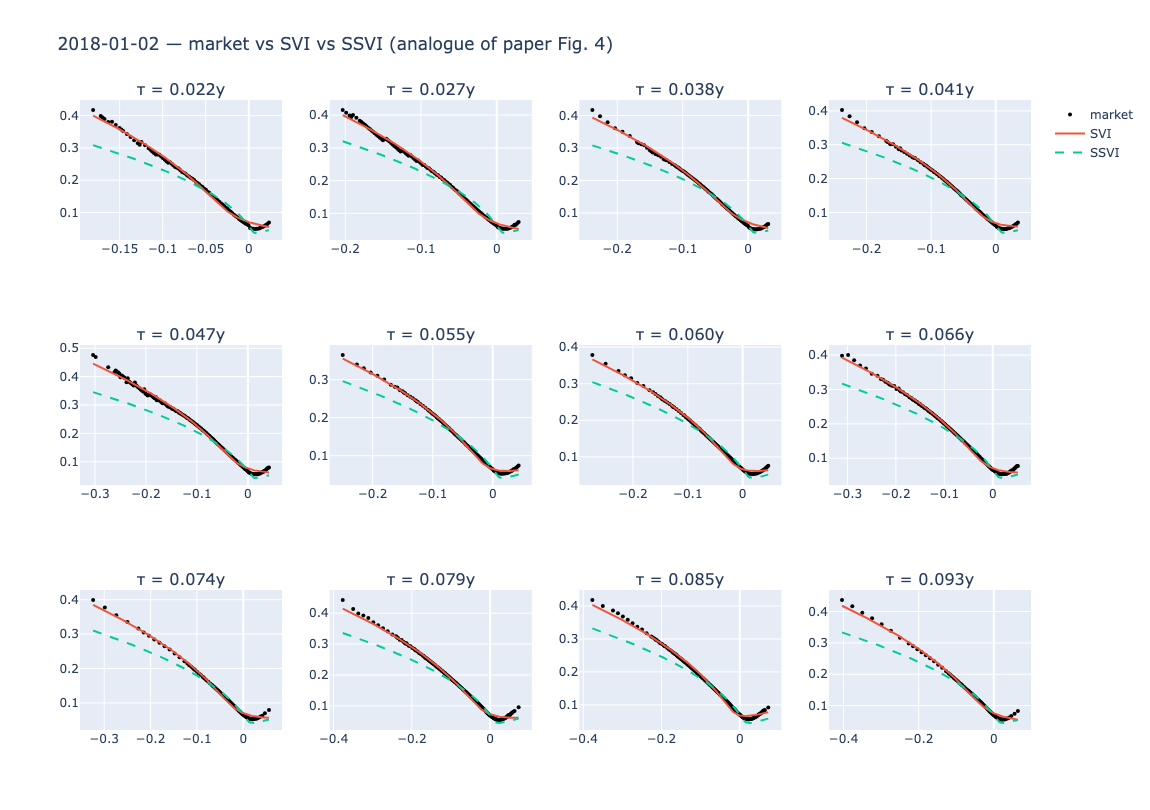
\includegraphics[
            width=1.3\textwidth,
            trim=0 0 0 2.5cm,
            clip
        ]{figures/nb02_c41_0.png}%
    }
    \caption{One representative trading day: market quotes (dots) with the per-slice SVI fit
    (solid) and the surface SSVI fit (dashed), the analogue of the paper's Fig.~4. Source:
    Notebook~02, cell~41.}
    \label{fig:nb02day}
\end{figure}

\begin{figure}[H]
    \centering
    \makebox[\textwidth][c]{%
        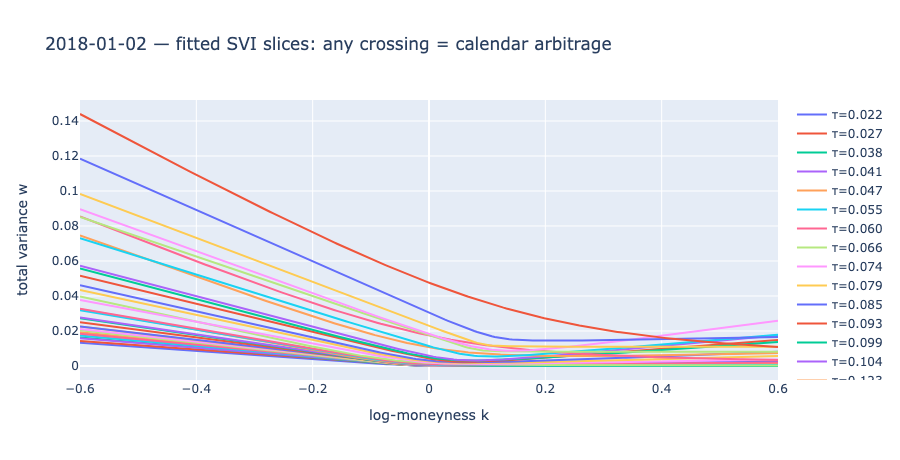
\includegraphics[
            width=0.8\textwidth,
            trim=0 0 0 2.5cm,
            clip
        ]{figures/nb02_c43_0.png}%
    }
    \caption{The same day's fitted SVI slices in total variance; any crossing is a calendar
    arbitrage between adjacent per-slice fits, the incoherence SSVI avoids by construction.
    Source: Notebook~02, cell~43.}
    \label{fig:nb02crossing}
\end{figure}




% ============================================================================
\section{Derivative-constrained deep smoothing and the collocation blind spot}
\label{sec:deep}
% ============================================================================

\subsection{Method}

Following \cite{ackerer2020}, the surface is the prior-corrector model \eqref{eq:arch}: an SSVI
prior with power-law term structure fitted to the day's quotes, multiplied by a positive
corrector ($2\times64$ tanh units, $\approx1$ at initialisation so that training \emph{starts at
the prior}). The prior is calibrated inside the Gatheral--Jacquier region, so by
Theorem~\ref{lem:range} it carries a printed certificate; on the synthetic experiments it reads
$\theta_{\max}=0.062$ with condition values $0.28<4$ and $0.83\le4$.

The loss is \eqref{eq:loss} with $\lambda_{\mathrm b}=\lambda_{\mathrm c}=10$,
$\lambda_{\mathrm w}=0.1$, and IV-targeted fit weights $\omega_i\propto1/(4w_i\tau_i)$, the same
weights as the calibrators of Section~\ref{sec:parametric} so that the cross-family comparison
is symmetric. All penalty derivatives are obtained by exact automatic differentiation and
validated against closed forms.

\subsection{Equal-epoch ablations on synthetic ground truth}

Ground truth is a known SSVI surface; the quotes are sparse (54 over six maturities), irregular
and noisy; and the prior is refit \emph{from the quotes}, so it is deliberately misspecified.
Four variants train for the same number of epochs with persistent optimiser state.

\begin{table}[H]\centering\small
\caption{Equal-epoch ablation ($800$ epochs). RMSE is measured against the dense truth at the
quoted maturities; the audit uses the independent extended grid.
\notebookfig{03}{equal-epoch dynamics}}
\label{tab:ablation}
\begin{tabular}{lccc}
\toprule
Variant & RMSE (\vp) & $\min g$ (audit) & bfly / cal violations \\
\midrule
full (prior $+$ penalties)  & 0.096 & $+0.310$ & 0\% / 0\% \\
no constraints              & 0.094 & $+0.311$ & 0\% / 0\% \\
no prior ($+$ penalties)    & 1.060 & $+0.268$ & 0\% / 0\% \\
no prior, no constraints    & 1.060 & $+0.268$ & 0\% / 0\% \\
\midrule
prior only (no corrector)   & 0.154 & n/a & 0\% / 0\% \\
\bottomrule
\end{tabular}
\end{table}

Two features of Table~\ref{tab:ablation} are worth noting. The two \emph{no-prior} rows are
identical to the last digit, and their training traces coincide exactly
(Figure~\ref{fig:nb03dynamics}). This equality is expected rather than a copy-paste error: on clean data
$g_\theta>0$ holds throughout training, so $\relu(-g_\theta)^2$ and its gradient vanish
\emph{exactly}, and the penalised and unpenalised runs follow the same trajectory. Second, the
certified prior carries the accuracy: $0.154\,\vp$ for the prior alone, $0.096\,\vp$ with the
corrector, against $1.06\,\vp$ with no prior. On clean data the prior provides most of the
protection, while the penalties remain inactive. To find out whether the penalties do anything at
all, we therefore need a stress case that induces arbitrage.

\begin{figure}[H]
    \centering
    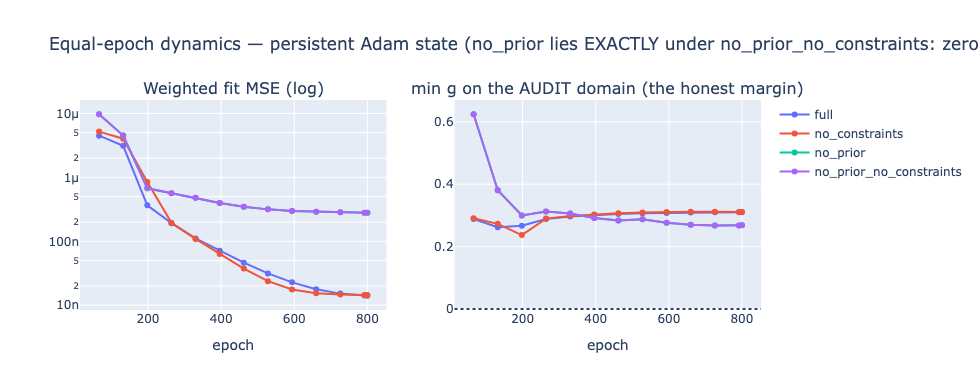
\includegraphics[width=0.92\textwidth,trim=0 0 0 2.5cm,clip]{figures/nb03_equal_epoch_dynamics.png}
    \caption{Equal-epoch training dynamics. Only three of the four traces are visible:
    \texttt{no\_prior} lies pixel for pixel beneath \texttt{no\_prior\_no\_constraints}, since
    with $g_\theta>0$ throughout training the penalty gradient vanishes identically and the two
    runs are the same computation. The near-coincidence of \texttt{full} and
    \texttt{no\_constraints} is by contrast only approximate, the residual gap being what the
    penalties charge on data that never demands arbitrage. Source: Notebook~03.}
    \label{fig:nb03dynamics}
\end{figure}


\subsection{A stress test that is guaranteed, fittable and gated}\label{sec:stress}

We deflate the last maturity slice by a factor $0.45$. Since
$0.45<\theta(0.9)/\theta(1.4)\approx0.657$, the deflated quotes sit strictly below those of the
previous maturity, so \emph{any} surface fitting both must have $\partial_\tau w<0$ somewhere
between them; the data-level crossing is $+0.0290$ in $w$. The stressor is therefore verified
analytically to force the pathology rather than assumed to. Deflation is chosen over inflation
because the IV-target weights \emph{raise} the stressed slice's weight and the corrector feature
required is low-frequency. A synthetic \emph{butterfly} stressor is deliberately absent: at
short maturities $g<0$ is driven by $w'^2/(4w)$ with tiny $w$, and would require distortions
sharper than a smooth prior-times-corrector can produce at fittable widths. The butterfly
penalty is instead ablated on real quotes in Section~\ref{sec:realablation}.

A stress comparison is interpretable only if the model actually \emph{fits} the stressor: if it
does not, apparent arbitrage violations may simply reflect poor convergence. Validity is
therefore verified by a two-condition gate on the unconstrained model: the deflated-slice RMSE
must be below $1\,\vp$, \emph{and} the fitted surface must reproduce at least half the
data-level crossing. The first alone would be insufficient, since a surface can graze the
deflated slice from above without ever crossing. The gate reads \texttt{PASS/PASS}, with
$0.069\,\vp$ and a fitted crossing of $+0.0296$ against $+0.0290$ in the data.

\subsection{The blind spot: exhibit, mechanism, repair}\label{sec:blindspot}

\paragraph{Exhibit.} On this gated stress, an early version of the smoother produced, for the
constrained model ($\lambda=10$), the following unexpected result:
\[
\texttt{pen\_cal}\big|_{\hat X_{\mathrm c}} \approx 0,
\qquad\text{while}\qquad
\text{audit-grid calendar violations}=28\%.
\]
Both were true. Diagnostics excluded the optimiser, since the constrained run had the
\emph{lower} total loss under its own objective, and excluded automatic differentiation, since
the $\tau$-path gradient was $0.25$ at a violating point and the $\tau$-derivative validated to
$10^{-11}$. What remained was the grid.

\paragraph{Mechanism.} The collocation followed the literature's prescription: exponentially
spaced maturities, dense at the short end where the butterfly constraint bites
\cite{ackerer2020}. With ten nodes on $[0.06,1.4]$ there is \emph{no node at all} between
$0.987$ and $1.400$, a $0.41$-year hole covering $30\%$ of the axis
(Figure~\ref{fig:gridhole}), exactly where the stressor forces the crossing. The optimiser
satisfied the penalty at every node and let the surface dip between them, which is precisely the
extremal configuration of Theorem~\ref{prop:nodegap}; the penalty therefore remained zero despite
violations between grid points. Using the same exponential grid for both constraints leaves the
calendar penalty poorly resolved at long maturities, which is \cite{chataigner2020}'s caveat in
its most literal form. This was detectable only because the audit grid is independent of, and
finer than, the collocation grid (Remark~\ref{rem:sampling}).

\paragraph{Repair.} The butterfly penalty keeps its ATM-dense grid (maximal gap $0.10$y); the
calendar penalty, which costs only one first derivative per node, gets its own uniform grid of
$80$ nodes with maximal gap $0.017$y. By Theorem~\ref{prop:nodegap} that is roughly a $24$-fold
reduction of the worst admissible hidden violation at equal curvature. A resolution assertion
verifies, before any stress run, that the calendar grid can actually see the stressed interval.

\begin{table}[H]\centering\small
\caption{Calendar stress, $\lambda$-sweep (final run, gated). ``mat'' denotes material violations
at $\mathrm{tol}_{\mathrm{mat}}=10^{-3}$ (Definition~\ref{def:materiality}). Node and audit
penalties now agree to grid noise. \notebookfig{03}{lambda sweep log}}
\label{tab:sweep}
\begin{tabular}{lcccc}
\toprule
$\lambda$ & deflated fit (\vp) & fitted crossing & cal.\ viol.\ strict (mat) & pen.\ nodes / audit \\
\midrule
0  & 0.069 & $+0.0296$ & 34.7\% (34.4\%) & $1.35\text{e-}3$ / $1.29\text{e-}3$ \\
1  & 1.991 & $+0.0000$ & 4.4\% (0.0\%)   & $1.3\text{e-}9$ / $1.2\text{e-}9$ \\
10 & 1.963 & $-0.0002$ & 1.6\% (0.0\%)   & $8.4\text{e-}11$ / $1.2\text{e-}10$ \\
\bottomrule
\end{tabular}
\end{table}

\paragraph{Result.} The unconstrained model follows the deflated quotes down, with a fitted
crossing of $+0.0296$ and material violations on a third of the audit domain; the constrained
model does not follow the deflated quotes, with a fitted crossing of $-0.0002$, at a measured
price of about $1.9\,\vp$ on the deflated slice. Material violations fall from $34.4\%$ to $0.0\%$. The
residual \emph{strict} rate of $1.6\%$, whose deepest residual is
$\partial_\tau w=-1.3\times10^{-4}$, is a residual effect of using soft rather than hard
constraints: reduced but not abolished, and now \emph{sized} rather than merely counted.

\begin{figure}[H]
    \centering
    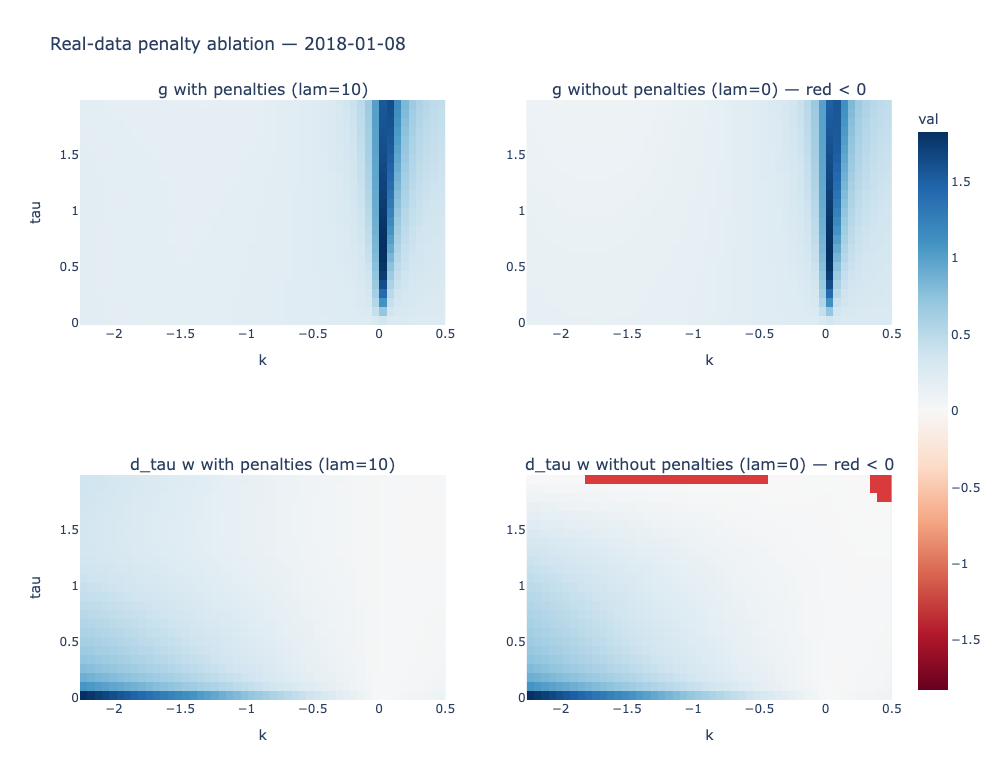
\includegraphics[width=0.92\textwidth,trim=0 0 0 2.5cm,clip]{figures/nb03_stress_A.png}
    \caption{The calendar stress under both regimes. The upper panels show $g$ and the lower
    panels $\partial_\tau w$, with and without penalties; red marks negative values, on a colour
    scale shared by both quantities. Without penalties (lower right) $\partial_\tau w$ turns
    negative in a band at the long end, at and beyond the last collocation node $\tau=1.4$, where
    the exponential grid places no node at all and the penalty therefore has nothing to enforce;
    with penalties (lower left) the surface holds $\partial_\tau w\ge0$ across the whole audit
    domain. The butterfly direction stays clean in both regimes. The $1.9\,\vp$ cost of that
    constraint is read off the deflated slice in Table~\ref{tab:sweep}.}
    \label{fig:nb03stress}
\end{figure}

\begin{finding}[The collocation blind spot]\label{find:blindspot}
A soft no-arbitrage penalty is a statement about its sampling set. A grid optimal for one
constraint can be structurally blind to another, the failure is invisible to the training loss
exactly, and it is detectable only by an audit grid independent of every collocation grid,
compared on a materiality scale. Constraint-specific collocation closes it.
\end{finding}

\subsection{Robustness to sparsity}\label{sec:sparsity}

Subsampling the quotes from $100\%$ to $50\%$ and then $25\%$, against per-slice SVI, exposed in
sequence two failures of \emph{our own} experimental design. Both are reported because each
produced an implausible result that revealed a problem in the experimental design.

The first was a data leak: the prior, collocation and input scaling were calibrated on the
\emph{full} quote set inside the subsampling loop, so the deep model kept seeing quotes SVI was
denied, and its RMSE \emph{fell} as $74\%$ of the data was removed. The second was an estimator
failure: one $50\%$ draw exploded to $14.2\,\vp$, because the naive ATM interpolation clamps on
one-sided slices and corrupts $\theta(\tau)$, and for a multiplicative corrector a \emph{wrong}
prior is worse than a \emph{flat} one ($14.2$ against $1.7\,\vp$), exactly as the
log-decomposition of \eqref{eq:arch} predicts. The robust nearest-ATM calibrator fixed it, and
the study became multi-seed with the prior-only RMSE printed for every draw, the diagnostic that
separates prior failures from corrector failures.

The deep smoother then degrades gracefully, $0.096\to0.22\to0.34\,\vp$, bounded below by the
prior-only curve. SVI first loses accuracy and then \emph{coverage}: at $25\%$ no slice retains
the six quotes a five-parameter SVI needs. Since SVI's RMSE is conditional on a calibrability
set that itself changes with the subsampling fraction, the comparison is \emph{paired} on the
same slices, draw by draw; the deep smoother wins $4/4$, including $0.137$ against
$1.615\,\vp$. One $25\%$ draw still degrades to $1.68\,\vp$, and its prior-only column of
$1.21\,\vp$ indicates that the degradation comes mainly from the prior rather than the corrector.

\begin{finding}[Sparsity robustness is inherited]\label{find:sparsity}
The deep smoother's robustness to sparse quotes is inherited from the calibration robustness of
its prior. The prior-times-corrector architecture moves the failure point; it does not remove it.
\end{finding}

\subsection{Real SPX days and the penalty ablation}\label{sec:realablation}

The per-day driver reuses the NB02 protocol and was staged on early-January 2018 days together
with an \emph{ex-ante} stress candidate selected from Section~\ref{sec:parametric}'s audit,
2018-01-08, which carries six butterfly-violating SVI slices with $\min_k g=-0.071$. On these
days the staging run returns a hold-out of $1.70$--$1.81\,\vp$, zero strict violations on both
domains, no blind flags, and a valid certificate every day. The $\gamma\le\tfrac12$ episode of
Remark~\ref{rem:cert} was diagnosed here, the per-day prior-only RMSE being what localised it,
and endpoint certification recovers the free fit: hold-out improves to $1.15$--$1.31\,\vp$.

\begin{figure}[H]
    \centering

    \begin{minipage}[t]{0.49\textwidth}
        \centering
        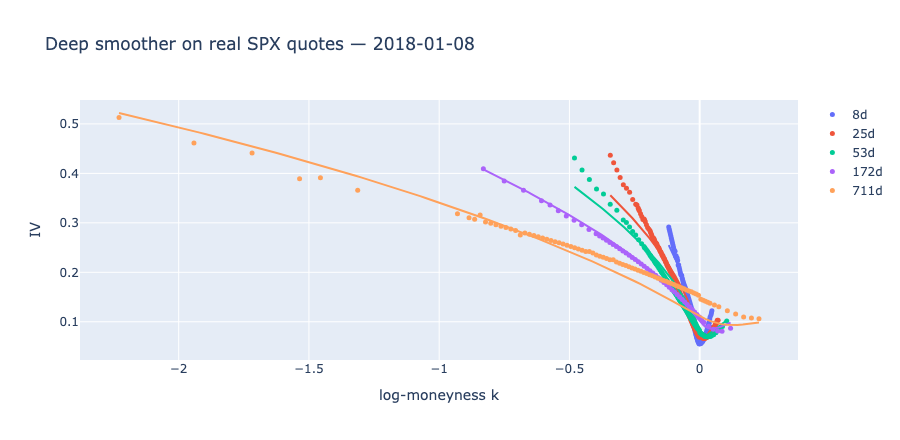
\includegraphics[
            width=\textwidth,
            trim=0 0 0 2.5cm,
            clip
        ]{figures/nb03_real_spx_quotes.png}
        \caption{The deep smoother on real SPX quotes, 2018-01-08: market quotes with the fitted
        surface, on the day carrying the worst butterfly violation of the parametric benchmark.
        Source: Notebook~03.}
        \label{fig:nb03real}
    \end{minipage}
    \hfill
    \begin{minipage}[t]{0.49\textwidth}
        \centering
        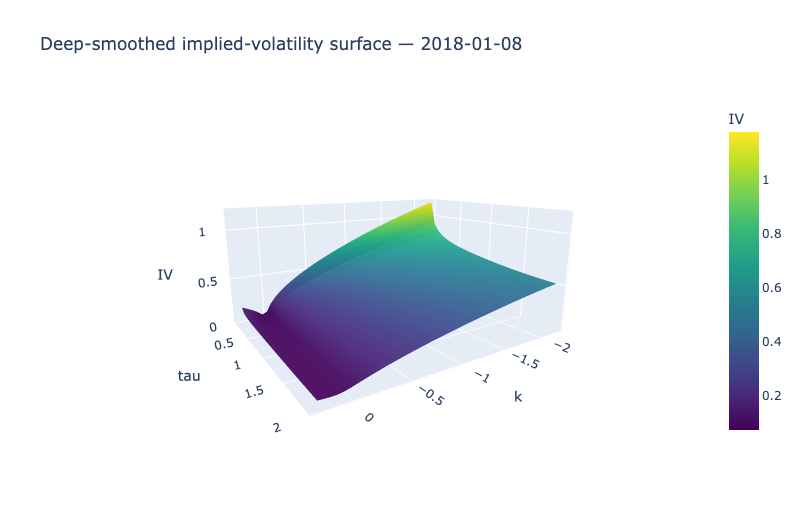
\includegraphics[
            width=\textwidth,
            trim=6cm 3cm 0 3.5cm,
            clip
        ]{figures/nb03_deep_smoothed_surface.png}
        \caption{The corresponding deep-smoothed implied-volatility surface for 2018-01-08.
        Source: Notebook~03.}
        \label{fig:nb03realsurface}
    \end{minipage}

\end{figure}


\paragraph{Which constraint binds on real data?} Refitting the stress-candidate day with
$\lambda_{\mathrm b}=\lambda_{\mathrm c}=0$, at identical seed and epoch budget, answers the
question. The butterfly penalty is \emph{identically zero at both} values of $\lambda$: with the
certified prior the surface never goes butterfly-negative even when unconstrained, so NB02's
$82.8\%$ ultra-short violation rate is a statement about raw per-slice SVI, not about this
architecture. The binding
real constraint is the \emph{calendar} one: on 2018-01-03, $\lambda=0$ leaves $19.1\%$ of the
extended domain violating with $\min\partial_\tau w=-0.25$, against $0.0\%$ at $\lambda=10$;
while on the most butterfly-stressed day the calendar penalty is also inactive and the prior
alone suffices. The hypothesis that real ultra-short quotes are the natural butterfly stressor
is thereby downgraded to a question for the full-sample production run, with the Volmageddon and COVID
weeks the natural suspects.

% ============================================================================
\section{Operator deep smoothing: one model for every surface}\label{sec:operator}
% ============================================================================

Section~\ref{sec:deep} fits one network per day; this section learns the smoothing \emph{map}
itself. Following \cite{wiedemann2025}, an operator $\mathcal G_\vartheta$ consumes a day's
quote cloud and returns $\widehat\sigma_{\mathrm{IV}}$ at any query point, for any day, with no
per-day optimisation. Three questions organise the section: what the operator programme delivers
in the \emph{academic-data} regime, one index and $1{,}926$ days, against the reference paper's
decade of proprietary multi-asset data; whether synthetic pretraining closes the gap; and
whether the operator's soft constraints survive the audit of Finding~\ref{find:blindspot}.

\subsection{Design}

The real bank holds the $1{,}926$ cleaned days, split chronologically into $1{,}155/385/386$ as specified in Section~\ref{sec:splits}, so every test number below is a temporal generalisation claim. The
synthetic bank holds $1{,}000$ SSVI surfaces with certified parameters and irregular quote
configurations, an unlimited arbitrage-free pretraining source.

We train a DeepONet-class operator \eqref{eq:deeponet} ($67{,}009$ parameters) and a
graph-neural-operator variant \eqref{eq:gno} ($34{,}697$ parameters), each under three regimes:
\textbf{R1} real-only, \textbf{R2} synthetic-only with zero-shot transfer, and \textbf{R3}
synthetic pretraining followed by real finetuning. Penalties are resolved by finite differences
on a $22\times9$ grid. That coarse grid is \emph{deliberately kept} as in the reference design,
because the gap between what it sees and what an independent audit sees is itself one of this
thesis's measurements.

Two engineering failures are worth reporting. The DeepONet trained from scratch on real data
collapsed to a constant: the training loss sat at exactly $1.0000$, the value of the relative
loss for a zero prediction, and the audit returned $\min g=0.9995$, the value $g\equiv1$ takes
for a surface flat in $k$. Real SPX days are dominated by far-OTM puts whose near-zero vegas
explode the normalised weights, driving the pre-activation far negative until the softplus
gradient vanishes; output-bias initialisation, a weight cap and a lower learning rate cure it.
The second failure follows from the first: the collapsed model displayed \emph{perfect}
discretisation invariance, because a constant is trivially invariant to its inputs
(Definition~\ref{def:discinv}). The invariance study is therefore \emph{gated} on fit validity,
the same epistemic move as the stress gate of Section~\ref{sec:stress}.

\subsection{Accuracy and transfer}

On the $386$ out-of-sample days the graph operator is the accuracy leader, reaching
$1.62\,\vp$ in R1 and $1.26\,\vp$ in R3, while the DeepONet depends on the synthetic
curriculum: $6.47\,\vp$ zero-shot in R2 against $2.20\,\vp$ in R3. The transfer question
therefore receives a qualified answer. Pretraining on certified synthetic surfaces closes most of
the zero-shot gap, $6.47$ to $2.20\,\vp$, so certified synthetic surfaces do carry usable
structure into the real problem; and unlike the DeepONet, the graph operator does improve on its
real-only run under the curriculum, $1.62$ to $1.26\,\vp$. But zero-shot synthetic-to-real
remains roughly three times worse than finetuned. The sim-to-real gap is real and finetunable
rather than absent.

Gated on fit validity, discretisation invariance holds well: the graph operator's dense-surface
shift under subsampling stays below $0.16\,\vp$ with only $25\%$ of inputs retained. The
amortisation argument is quantified directly: $0.8$--$0.9$\,ms per surface for the DeepONet and
$39$--$413$\,ms for the graph operator on CPU, against roughly $80$--$100$\,s per day for the
Section~\ref{sec:deep} smoother and about $1$\,s for SVI.

\begin{figure}[H]
    \centering
    \makebox[\textwidth][c]{%
        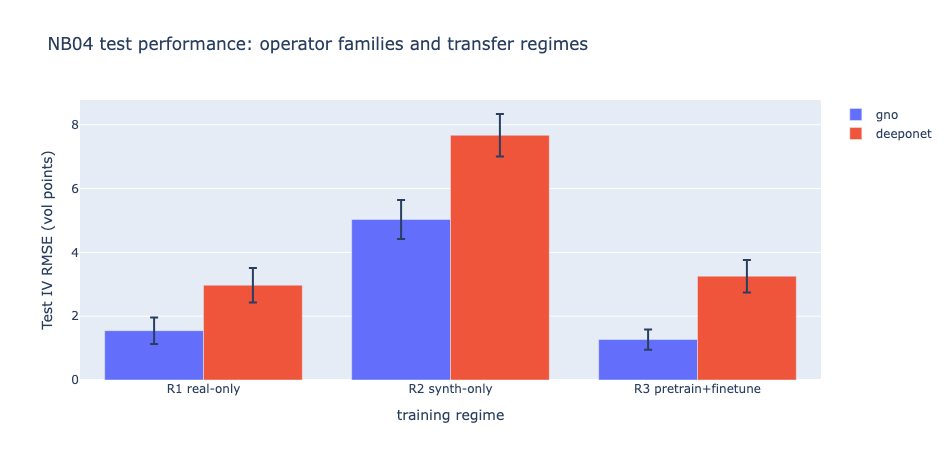
\includegraphics[width=0.8\textwidth]{figures/nb04_c09_2.png}
    }
    \caption{Hold-out IV RMSE across families and transfer regimes on the $386$ out-of-sample
    days, the same metric reported in Table~\ref{tab:opaudit}. Synthetic pretraining followed
    by real finetuning (R3) improves both families, and rescues the DeepONet from its zero-shot
    R2 performance; the graph operator leads on fit in every regime. Source: Notebook~04,
    cell~9.}
    \label{fig:nb04transfer}
\end{figure}

\begin{figure}[H]
    \centering
    \makebox[\textwidth][c]{%
        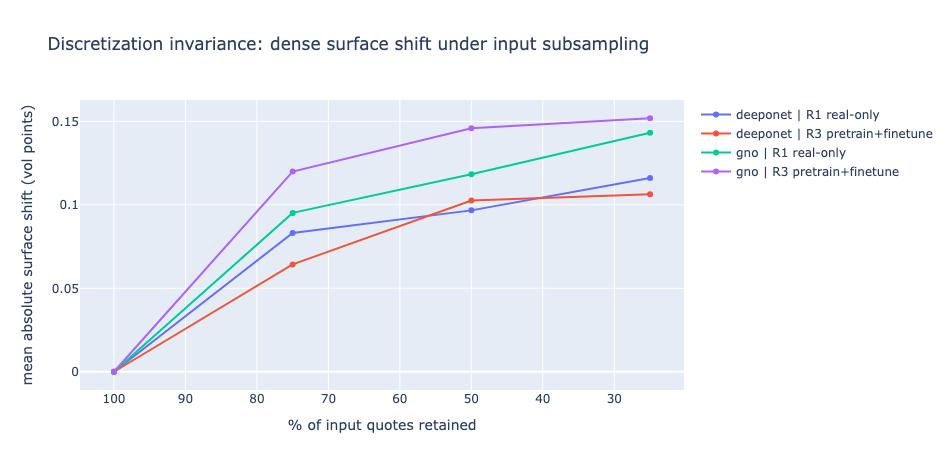
\includegraphics[
            width=0.8\textwidth,
            trim=0 0 0 2.5cm,
            clip
        ]{figures/nb04_c11_0.png}
    }
    \caption{Discretisation invariance, gated on fit validity: dense-surface shift under input
subsampling, for the real-only and finetuned regimes. The zero-shot synthetic-only regime is not
shown: its fits are the weakest of the study ($6.47$ and $4.79\,\vp$), and the stability of a
surface that fits the market poorly answers a different question from the one asked here.}
    \label{fig:nb04invariance}
\end{figure}

\newpage
\subsection{The audit: the blind spot is transversal}\label{sec:opaudit}

Every penalty is evaluated twice: on the \emph{penalty grid} ($22\times9$, maximal $\tau$-gap
$0.176$y, the grid the optimiser saw) and on an \emph{independent audit grid} ($61\times31$,
uniform, disjoint nodes), with strict and material rates and per-day blind flags. Restricting the audit to the convex hull of the quoted domain, which covers $77\%$ of the box,
does not rescue the result: the graph operator's material butterfly rate is $22.1\%$
hull-restricted in R1 and $21.9\%$ in R3, essentially unchanged.

\begin{table}[H]\centering\small
\caption{Operator audit on the $386$ out-of-sample days: material violation rates on the
independent $61\times31$ grid, blind-spot days (materially clean on the penalty grid, materially
violating on the audit grid), the worst audit $g$, and the number of days passing the $5\,\vp$
fit gate. Penalty-grid rates, which are what the training loss reports, are near zero throughout.
\notebookfig{04}{operator summary table}}
\label{tab:opaudit}
\begin{tabular}{llccccccc}
\toprule
Model & Regime & Hold-out & \multicolumn{2}{c}{Audit material viol.}
 & \multicolumn{2}{c}{Blind days /386} & $\min g$ & Fit gate \\
\cmidrule(lr){4-5}\cmidrule(lr){6-7}
 & & (\vp) & bfly & cal & bfly & cal & (audit) & /386 \\
\midrule
DeepONet & R2 synth-only & $6.47$ & $0.000\%$  & $0.000\%$ & 0   & 0   & $+0.241$ & $2^{\ast}$ \\
DeepONet & R1 real-only  & $2.69$ & $0.000\%$  & $0.056\%$ & 1   & 49  & $-0.003$ & 383 \\
DeepONet & R3 pre+fine   & $2.20$ & $0.008\%$  & $0.000\%$ & 25  & 0   & $-0.029$ & 383 \\
GNO      & R2 synth-only & $4.79$ & $23.35\%$  & $0.412\%$ & 303 & 275 & $-35.3$  & 218 \\
GNO      & R1 real-only  & $1.62$ & $21.17\%$  & $0.033\%$ & 356 & 79  & $-30.6$  & 386 \\
GNO      & R3 pre+fine   & $\mathbf{1.26}$ & $21.75\%$ & $0.067\%$ & 355 & 86 & $\mathbf{-32.6}$ & 386 \\
\bottomrule
\end{tabular}\\[2pt]
{\footnotesize $^{\ast}$ The synthetic-only DeepONet passes the fit gate on $2$ days out of
$386$, so its zero violation rates describe a surface that does not fit the market; by
rule~(A4) the row is reported but not read as a clean result.}
\end{table}

Table~\ref{tab:opaudit} is this section's central result, and the ordering of its first two
columns matters. The graph operator has the \emph{best hold-out fit in the entire thesis},
$1.26\,\vp$ in R3, and is simultaneously materially butterfly-violating on $21.75\%$ of the
independent audit domain, blind on $355$ of $386$ days, with a worst audit value of
$\min g=-32.6$. Its own penalty-grid audit reports near-zero. It passes the fit gate on
\emph{every} day, so the violations cannot be dismissed as the artefacts of a model that failed
to converge.

The same blind spot now appears in a second dimension. In Section~\ref{sec:deep} the penalty was blind
\emph{in space}, satisfied at the nodes and violated between them. Here it is blind in space
\emph{and in time}: the penalty was minimised on the training days' surfaces, and nothing
transports that property to test days, so the constraint does not generalise with the fit. The
contrast between the two architectures is the one predicted in Section~\ref{sec:opsec}.
The DeepONet is essentially immune in the butterfly direction when trained on real data, its
outputs lying in the span of a global smooth trunk basis (Proposition~\ref{thm:deeponet}); its
residual weakness is calendar, on $49$ blind days. The locally assembled graph operator, through
the same inductive bias that improves its accuracy (Remark~\ref{rem:gnobias}), produces
fine-scale curvature that a $22\times9$ finite-difference penalty cannot see and a $61\times31$
audit can.

One result was not anticipated: synthetic pretraining does not clean the DeepONet, it
\emph{moves} its failure. Real-only training leaves $49$ calendar-blind days and a single
butterfly-blind day; pretraining followed by finetuning leaves $25$ butterfly-blind days and no
calendar-blind day. The direction of the failure inverts while the fit improves only mildly
($2.69$ to $2.20\,\vp$), a warning against reading any single violation column in isolation:
improving one constraint during training can worsen the other.

\begin{figure}[H]
    \centering
    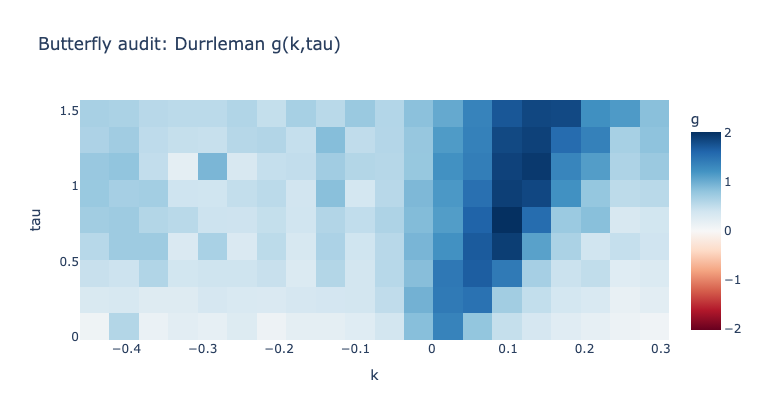
\includegraphics[width=0.92\textwidth]{figures/nb04_c12_2.png}
    \caption{Independent butterfly audit of the graph operator on the worst of its $355$ blind
    days (2024-05-10). The Durrleman function is evaluated on audit nodes disjoint from the
    $22\times9$ penalty grid; red marks materially negative cells, roughly a quarter of the
    domain, concentrated in the put wing and at the long end where quotes are sparse. The same
    day's penalty-grid audit reports materially clean. The colour scale is clipped at $\pm5$,
    and the worst value is not read off this figure: $\min g$ is an extreme order statistic
    carried by a single node, and is quoted in Table~\ref{tab:opaudit} at the audit's own
    resolution. Source: Notebook~04, cell~12.}
    \label{fig:nb04audit}
\end{figure}

\begin{figure}[H]
    \centering
    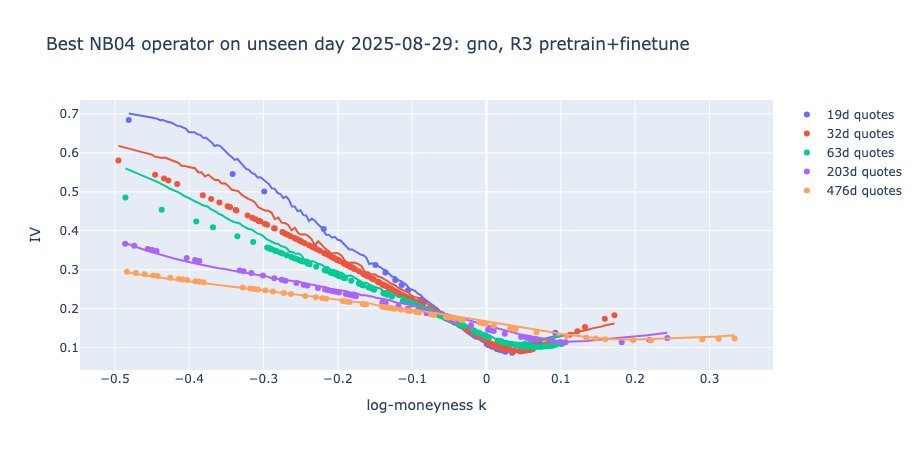
\includegraphics[width=0.92\textwidth,trim=0 0 0 2.5cm,clip]{figures/nb04_c12_0.png}
    \caption{The best operator on a genuinely unseen day (2025-08-29): the fit is reasonable but
    visibly coarser than the per-day smoother, which is the cost of amortisation. Source: Notebook~04,
    cell~12.}
    \label{fig:nb04unseen}
\end{figure}


\begin{finding}[The blind spot is transversal and two-dimensional]\label{find:transversal}
Soft no-arbitrage constraints fail to bind (i)~\emph{between collocation nodes} and, for
operators, (ii)~\emph{across days}, since enforcing them on training surfaces does not constrain
test surfaces. Reported violation rates are meaningful only relative to an audit grid
independent of the penalty grid \emph{and} a data split independent of training. Under that
standard, the most accurate operator in this study is also the one with the highest violation
rates, blind on $355$ to $356$ of $386$ unseen days, an inversion that its own training log does
not show.
\end{finding}

% ============================================================================
\section{Closing the gap: embedding the certified prior in the operator}
\label{sec:prioroperator}
% ============================================================================

The previous section identified the problem; this section tests a possible solution, and in
doing so resolves an inconsistency in the thesis as it stands: the deep smoother of
Section~\ref{sec:deep} uses a certified prior that demonstrably carries the protection
(Table~\ref{tab:ablation}), while the operators map the quote cloud \emph{directly} to the
surface with no prior anywhere. That was deliberate: the purpose of Section~\ref{sec:operator}
was to audit the \emph{published} design \cite{wiedemann2025}, and modifying the architecture
first would have made the violation rates a statement about our variant rather than about the
reference. Having completed that audit, we now ask whether the protective mechanism transfers.

\paragraph{Design.} For every day, an SSVI prior is fitted from that day's own quotes inside the
Gatheral--Jacquier region, so by Theorem~\ref{lem:range} it carries a printed certificate. The
operator then learns only a bounded multiplicative correction,
\begin{equation}\label{eq:prioroperator}
\widehat\sigma_{\mathrm{IV}}(k,\tau)\;=\;
\underbrace{\sigma_{\mathrm{SSVI}}(k,\tau)}_{\text{certified, per day}}\times
\exp\Bigl(\underbrace{s\,\tanh\bigl(\mathcal G_\vartheta(a)(k,\tau)\bigr)}_{\text{correction, }|c|\le s}\Bigr),
\qquad s=0.35,
\end{equation}
and the quote cloud enters through the log-residual
$\log(\sigma^{\mathrm{mkt}}_i/\sigma_{\mathrm{SSVI}}(k_i,\tau_i))$, so the operator sees
directly what the prior fails to explain. Four properties follow, each addressing something
Section~\ref{sec:operator} exposed.

\begin{enumerate}[label=(\roman*)]
\item \textbf{Training starts at the prior.} The correction head is zero-initialised, so
$c\equiv0$ at initialisation and the operator \emph{is} the certified SSVI surface, asserted
numerically before every run to $10^{-8}$.
\item \textbf{Positivity becomes structural.} The softplus head whose saturation caused the
collapse is no longer needed: positivity comes from a positive prior times an exponential.
\item \textbf{The correction is bounded}, $|c|\le s$: a curvature budget in the sense of
Theorem~\ref{prop:nodegap}. It does not prove $g\ge0$, but it bounds how far the operator can
travel from a surface that satisfies it.
\item \textbf{Inheritance.} Wherever the correction is flat, all derivatives of the output are
the prior's, and the prior carries a theorem.
\end{enumerate}

Prior-times-correction is a strong inductive bias, \emph{not} a guarantee: a correction with
enough curvature can still drive $g$ negative within its budget. The result below is therefore
reported as a measured reduction under an identical audit, never as a certificate.

The comparison is like for like: same regimes, split, loss weights, penalty grid and audit
grid; only the architecture differs. One caveat is disclosed: the synthetic bank is generated
\emph{from} SSVI, so a fitted prior recovers it almost exactly and leaves the corrector nothing
to learn. The prior-embedded families therefore pretrain on a perturbed synthetic bank, and the
headline comparison is R1 against R1, which is unaffected by that choice.

\begin{table}[H]\centering\small
\caption{Effect of embedding the certified prior, real-only regime (R1), on the $386$
out-of-sample days. Audit columns are material rates on the independent $61\times31$ grid.
\notebookfig{04}{operator summary table, prior families}}
\label{tab:prioroperator}
\begin{tabular}{lcccccc}
\toprule
Model & Hold-out & Audit bfly & Audit cal & Blind days & $\min g$ & Fit gate \\
 & (\vp) & (mat) & (mat) & (bfly/cal) & (audit) & /386 \\
\midrule
DeepONet                & $2.69$ & $0.000\%$ & $0.056\%$ & $1\,/\,49$ & $-0.0028$ & 383 \\
DeepONet $+$ prior      & $\mathbf{1.32}$ & $\mathbf{0.000\%}$ & $\mathbf{0.000\%}$
                        & $\mathbf{0\,/\,0}$ & $\mathbf{+0.071}$ & 386 \\
\midrule
GNO (R1)                & $1.62$ & $21.17\%$ & $0.033\%$ & $356\,/\,79$ & $-30.6$ & 386 \\
GNO (R3, best fit)      & $1.26$ & $21.75\%$ & $0.067\%$ & $355\,/\,86$ & $-32.6$ & 386 \\
GNO $+$ prior           & \multicolumn{6}{c}{\emph{not available: run terminated, see note}} \\
\bottomrule
\end{tabular}
\end{table}

The \texttt{gno\_prior} family did not yield a usable model: its training was terminated by a
mid-run process kill on the shared cluster and the state dictionary was never checkpointed, so
the $2\times2$ matrix is completed on three of its four cells. This does not weaken the
constructive claim, which is carried by the DeepONet row: the critique it answers, namely that
soft penalties do not transport across days, is architecture-agnostic.

\paragraph{Reading the result.} Read against Table~\ref{tab:opaudit}, the prior-embedded
DeepONet resolves the inversion rather than merely improving one column. Its hold-out error falls
from $2.69$ to $1.32\,\vp$, halving the gap to the accuracy leader, while both audit columns go
to exactly zero and $\min g$ crosses from $-0.0028$ to $+0.071$: not a single materially
violating cell on any of the $386$ days, against $49$ calendar-blind days for the plain DeepONet.
The butterfly direction was already essentially clean without the prior, so what the prior
removes here is the \emph{calendar} blind spot, the one direction in which the trunk basis of
Proposition~\ref{thm:deeponet} offers no protection.

The comparison that matters is with the graph operator. At $1.26\,\vp$ the GNO fits marginally
better, by $0.06\,\vp$, and pays for it with $21.75\%$ of its audit domain materially violating
and $355$ blind days. The difference in fit is only $0.06\,\vp$, while the prior-embedded model
is audit-clean on every out-of-sample day. Among operators that fit the
market at all, in the sense of rule~(A4), it is the only such surface: the synthetic-only
DeepONet of Table~\ref{tab:opaudit} is audit-clean too, but on a fit that clears the gate on two
days out of $386$.

\begin{finding}[The certified prior transfers from the smoother to the operator]
\label{find:prioroperator}
Embedding a per-day certified SSVI prior and learning only a bounded correction removes the
DeepONet operator's remaining blind spot entirely: its $49$ calendar-blind days and single
butterfly-blind day fall to zero, both material audit rates to $0.000\%$, and the worst audit
$g$ from $-0.0028$ to $+0.071$, across all $386$ out-of-sample days. It does so at
\emph{negative} cost in fit, halving the hold-out error from $2.69$ to $1.32\,\vp$, for a
per-day prior calibration of roughly one second. The resulting model sits within $0.06\,\vp$ of
the study's accuracy leader while being the only operator that is simultaneously audit-clean and
usable as a fit. The mechanism that protects the deep smoother therefore transfers to the
operator family. It remains an inductive bias rather than a guarantee, but on this data it
removes the pathology entirely rather than merely reducing it.
\end{finding}